\section{Entwicklungsstufen}
\subsection{Multiplikation}

Zeigen, welche Bits heraus genommen werden müssen! und belegen warum.

\subsection{Addierer}
CLA, RC, in einem Takt

\subsection{Konstantenmultiplikation}
Dieser Punkt muss irgendwie mit der Implementierung des Konstantenmultiplizierers zusammengeführt werden.

Der duale Wert lässt sich am einfachsten mit der Matlab-Funktion \texttt{fi()} ermitteln. Der Funktion werden hierfür Kommagetrennt der Deziamlwert, 1 für vorzeichenbehaftet,
die gesamte Anzahl an Stellen (13) und die Anzahl der Nachkommastellen (10) übergeben. Der vollständige Aufruf sieht dann wie folgt aus:

% \begin{lstlisting}[language=matlab, frame=false, numbers=none, keywordstyle=\color{black},rulecolor=\color{white}]
% val=fi(sqrt(2)/2,1,13,10)
% \end{lstlisting}
\texttt{val=fi(sqrt(2)/2,1,13,10)}

Der erzeugte Datentyp hat unter anderem die Eigenschaften \texttt{val.bin}, welche einem mit $0001011010100$ den Wert als Binärzahl zurück gibt, 
\texttt{val.double} gibt den approximierten Dezimalwert mit 0,70703125 zurück und \texttt{val.dec} interpretiert den Dualwert als Integer, was 724 entspricht.
Letzterer ist wichtig zu kennen, um die Werte der Simulation nachvollziehen zu können.

Der Berechnung aus Gleichung (\ref{eq:abweichungWurzel2halbe}) kann entnommen werden, dass die Abweichung weit unter einem Prozent liegt.

\begin{equation}\label{eq:abweichungWurzel2halbe}
 \frac{100}{\dfrac{\sqrt{2}}{2}}\cdot 0,70703125 = 99,989\%
\end{equation}



\subsection{1D-DFT mit Integer-Werten}
 
\subsection{2D-DFT mit Integer-Werten}

\subsection{2D-DFT mit Werten SQ-Format}

\subsection{Zusammenhang von DFT und IDFT bei der Matrixmultiplikation}

Durch die umgekehrte Drehrichtung des komplexen Zeigers in Gleichung (\ref{eq:idft}) werden in der Matrizenschreibweise die Zeilen 2 und 8, 3 und 7 sowie 4 und 6 vertauscht.
Nachvollziehen lässt sich das gut anhand der Grafik (\ref{pic:Einheitskreis_Faktoren}). 
Verdeutlicht wird das vorgehen in Abbildung \ref{pic:IDFT_Zeilentausch}.

\begin{figure}[ht]
 \centering
 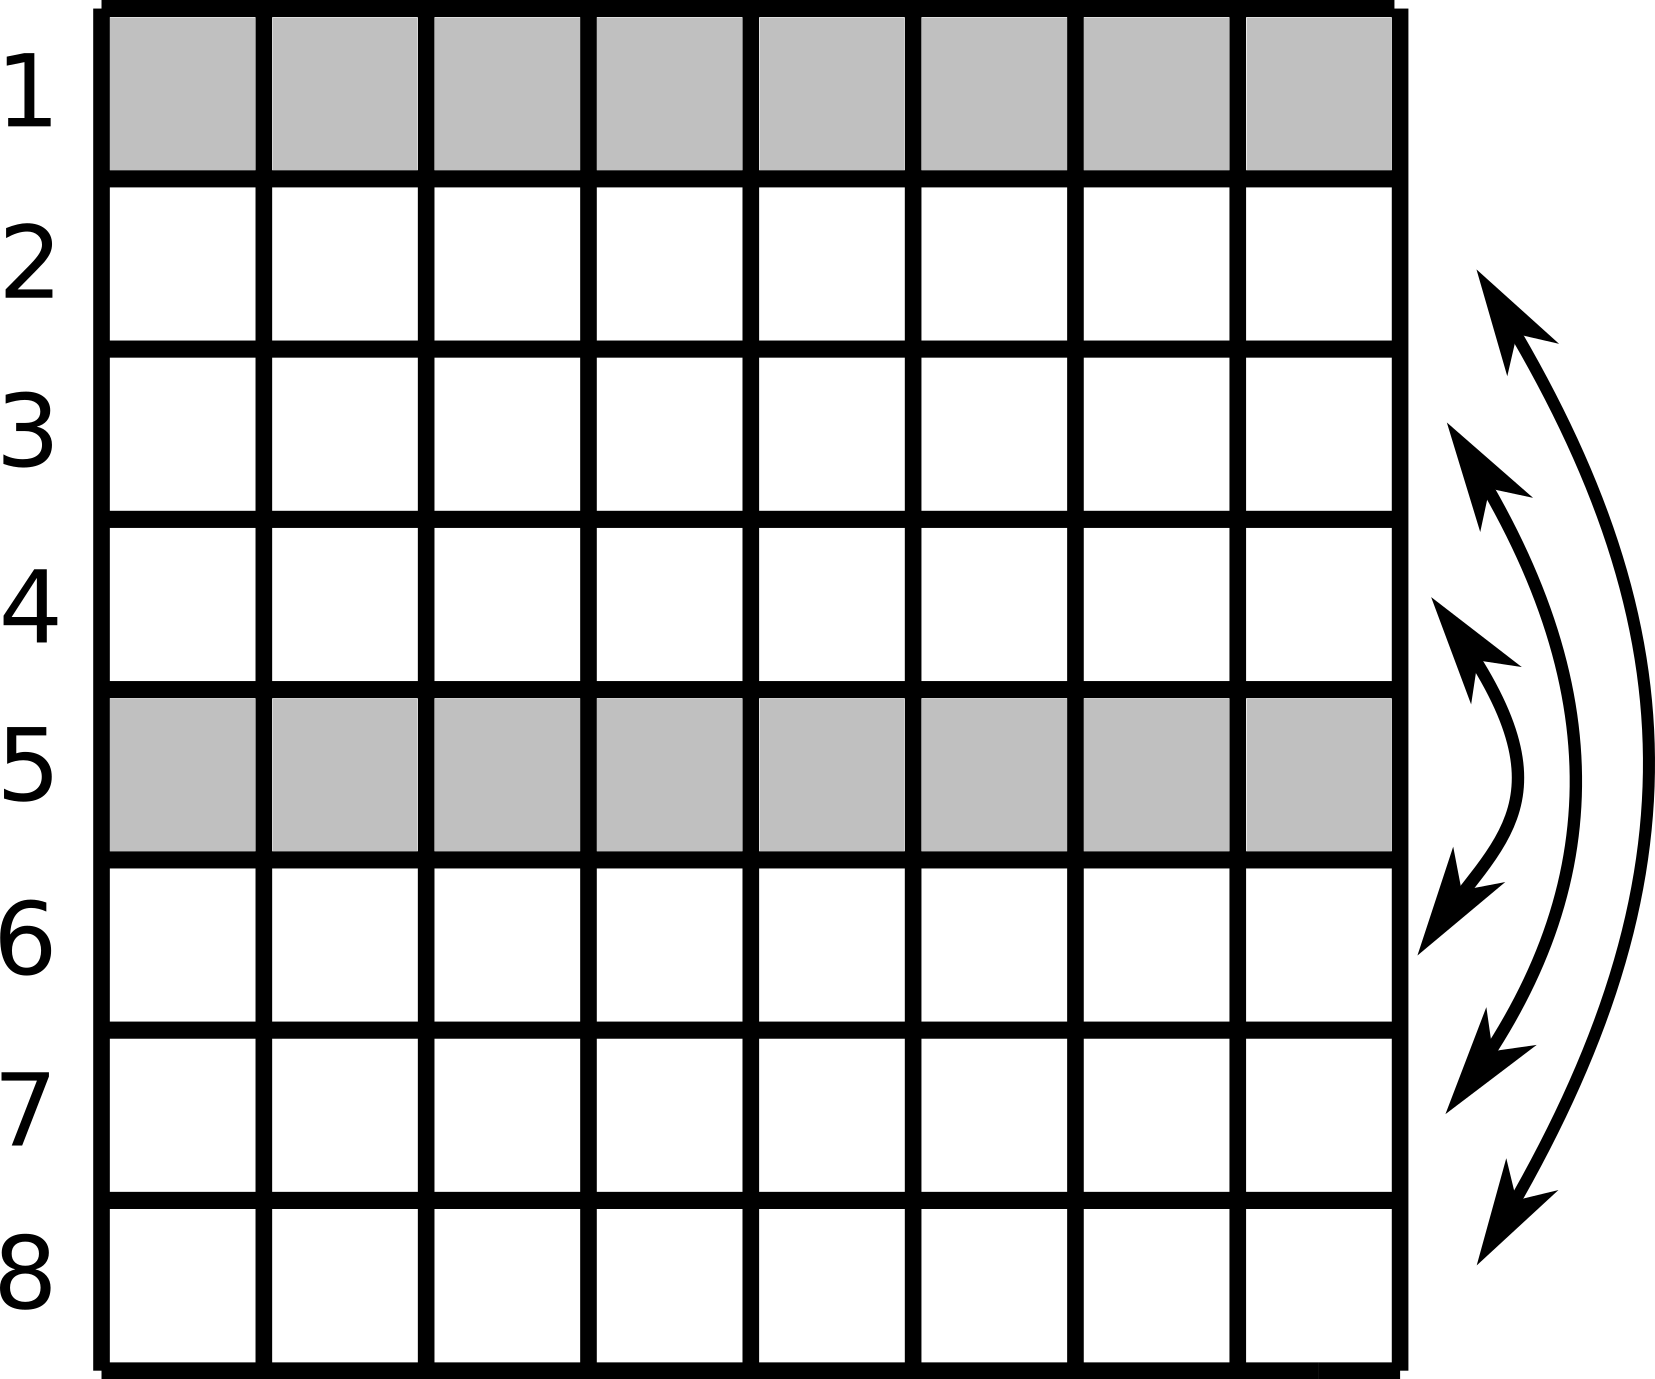
\includegraphics[width=0.4\textwidth]{img/IDFT_Zeilentausch.png}
 \caption{Um von der DFT zur IDFT zu kommen, müssen bei der Matrixmultiplikation die Zeilen 2 und 8, 3 und 7 sowie 4 und 6 der Twiddlefaktormatrix vertauscht werden}
 \label{pic:IDFT_Zeilentausch}
\end{figure}



\section{Test der Matrixmultiplikation}
Unter anderem weil NC\,Sim bzw. dessen Unterprogramm SimVision zur Anzeige von Signalverläufen (Waveform) nur Integer darstellen kann und bei als Vektor gebündelten Signalen 
diese nicht einmal als vorzeichenbehaftet (signed), wurde der Einfachheit halber zunächst die Berechnung als Ganzzahl-Multiplikation mit dem Faktor 3 betrachtet. 
Da es bei diesem Faktor und den gewählten Eingangswerten nicht zu einem 
Überlauf kommen kann, war es zu diesem Zeitpunkt noch nicht nötig, sich Gedanken über die Breite des Ergebnisvektors bzw. den Ausschnitt daraus für die weitere
Berechnung zu machen. Deshalb konnte an dieser Stelle noch auf den Bitshift zur Halbierung der Werte verzichtet werden.

Erst als der Faktor $\frac{\sqrt{2}}{2}$ übernommen wurde, wurden die Ergebnisse breiter als der Vektor für die weitere Berechnung an Bits zur Verfügung stellt.

${\frac{\sqrt{2}}{2}}_{10}$ = $0001011010100_2$ in S2Q10, als Integer betrachtet jedoch $724_{10}$.

Daraus folgt, dass ein Teil der Bits abgeschnitten werden müssen. Da die Dualzahlen jetzt im S1Q10-Format betrachtet werden, es sich also um Kommazahlen handelt,
müssen die hinteren Bits abgeschnitten werden. Zudem können vorne Bits ohne Informationsverlust gestrichen werden, da durch die Multiplikation ein weiteres 
Negations-Bit dazugekommen ist und auf Grund des gegebenen Faktors der Wertebereich vorne nie ganz ausgenutzt wird. (Verifizieren / Belegen!)


\section{Implementierung des Konstantenmultiplizieres}\label{sec:Konstantenmultiplizierer}

Anfangs wurde angenommen, dass Multiplikationen mit den Twiddlefaktoren $\pm 1$ und $\pm\frac{\sqrt{2}}{2}$ durchgeführt werden müssen. 
Dass bei einer optimierten 8x8-DFT wegen des explizieten ausprogrammierens der Berechnungen die Multiplikation mit $\pm1$ wegfällt, wurde recht schnell klar.
Erst bei genauer Betrachtung der Twiddlefaktor-Matrix viel auf, dass in jeder Zeile gleich viele Additionen wie Subtraktionen vorhanden sind. Durch Umsortieren 
ist es dadurch möglich auf das Invertieren der Eingangswerte sowie den hierfür benötigten Takt und die Inverter zu verzichten. Weiter wird auch nur die Multiplikation
mit $+\frac{\sqrt{2}}{2}$ benötigt.

\subsection{Syntheseergebnis eines 13 Bit Konstantenmultiplizierers}\label{sec:SyntheseergebnisKonstantenmultiplizierer}
\begin{figure}[!ht]
\centering  
 %\fbox{
  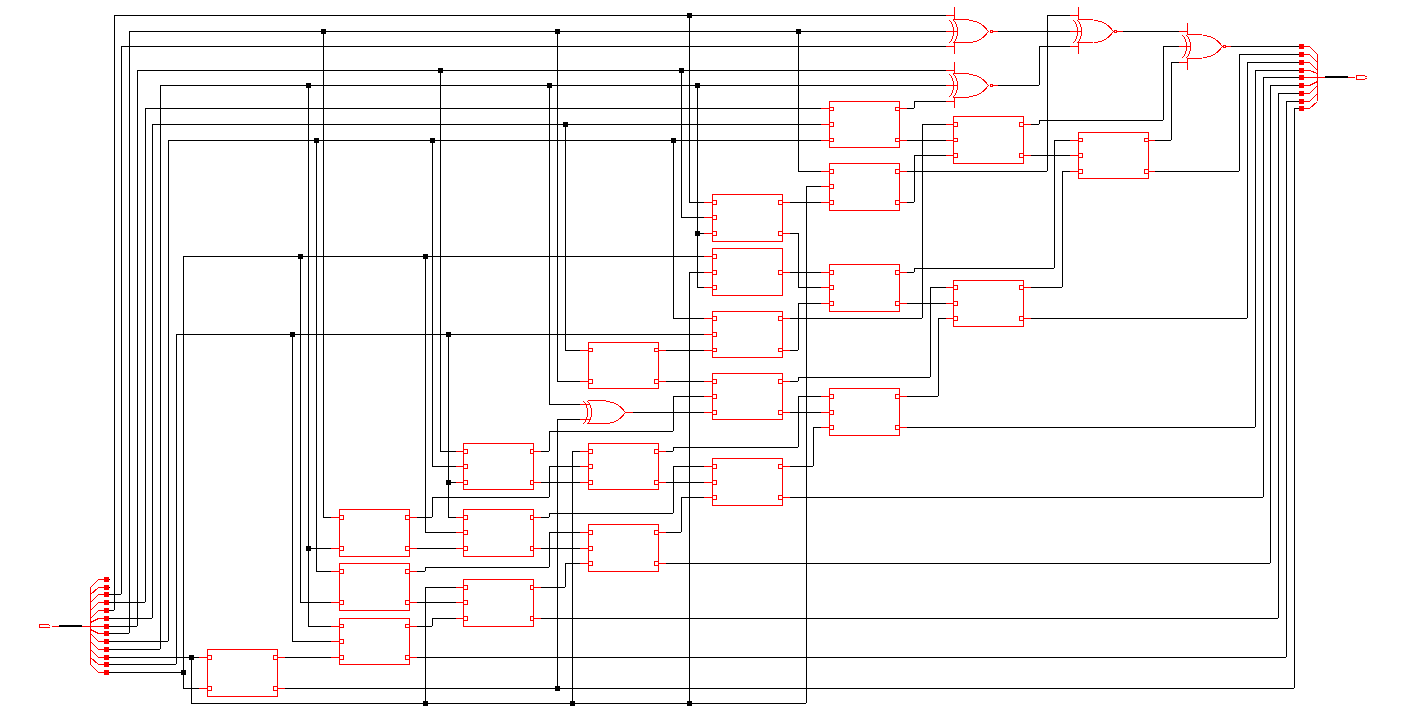
\includegraphics[width=1\textwidth]{img/13Bit_Konstantenmultiplizierer_Netlist.png}
  %}
  \caption{13 Bit Konstantenmultiplizierer für $\frac{\sqrt{2}}{2} = 0.70711 \simeq 0.70703125 = 0001011010100_2$ in Encounter; Eingang links, Ausgang rechts}
  \label{pic:Konstantenmultiplizierer}
\end{figure}



\begin{table}[!ht]
 \caption{Vergleich Konstanten- mit regulärem Multiplizierer}
 \label{tab:VergleichMultiplizierer}
 \begin{tabular}{ccc}
 \hline
				& Konstantenmultiplizierer 	& regulärer Multiplizierer\\
  \hline	
  Gatter			& 27				& 175 \\
  Fläche (Prozess: 350nm)	& $\SI{6612}{um^2}$		& $\SI{23261}{um^2}$\\
  \hline
 \end{tabular}
\end{table}





Der vollständige Gate-Report befindet sich in Abschnitt \ref{src:rc_gate_report} auf Seite \pageref{src:rc_gate_report}



\subsection{Syntheseergebnis für die Bildung des Zweierkomplements eines 13 Bit Vektors}\label{sec:SyntheseergebnisBildungZweierkomplement}

Zum Vergleich mit dem Konstantenmultiplizierers aus Abb. \ref{pic:Konstantenmultiplizierer} soll in Abb. \ref{pic:13BitInverter} die nicht expliziet implementierte aber in Abschnitt
\ref{sec:GegenüberstellungRelleKomplexeEingangswerte} erwähnte Negierung von Zahlen gezeigt werden.

\begin{figure}[htpb]
\centering
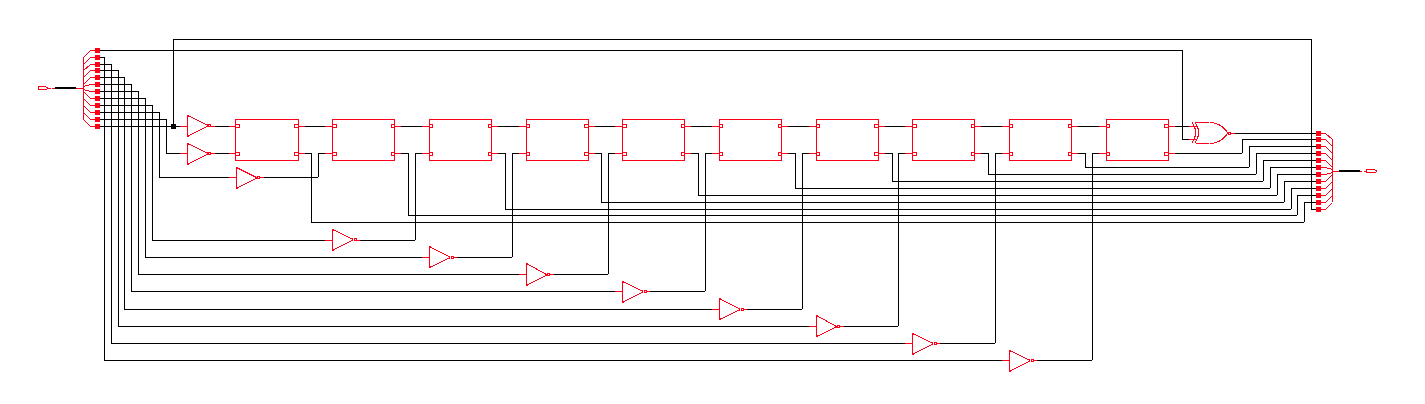
\includegraphics[width=0.99\textwidth]{img/13Bit_Inverter_Netlist.png}
\caption{Netzliste einer Einheit zur Bildung des 2er-Komplements eines 13 Bit Vektors; Eingang links, Ausgang rechts}
\label{pic:13BitInverter}
\end{figure}

Für die Negierung eines 13 Bit Vektors hat das Synthesewerkzeug \texttt{encounter} 22 Standardzellen verwendet. Das sind knapp doppelt so viele Gatter, wie der Vektor 
Bits breit ist. Der Unterschied zum Konstantenmultiplizierer fällt somit sehr gering aus. 
Wie zu sehen, handelt es sich fast ausschließlich um Inverter und Addierer. In Abschnitt \ref{sec:Integer2erKomplement} wurde bereits beschrieben, dass für die Bildung des
2er-Komplements zunächst alle Bits invertiert werden müssen. Abschließend wird auf den Vektor 1 LSB addiert. 
Beide Pfade weisen die gleiche Länge auf und verwenden überwiedend die selben
Gattertypen, weshalb darauf geschlossen werden kann, dass die maximale Gatterlaufzeit in der gleichen Größenordnung liegen muss.